\section{اثبات \autoref{theorem:mainResult}}
\label{sec:ProofmainResult}
برای اثبات 
\gls{UpperBound} به \cite{Feder1994Relations,Hu2012Analytical}
مراجعه کنید. برای 
\gls{LowerBound}
فرض کنید که 
$k\longrightarrow  Y \longrightarrow \hat{k}$ یک \gls{MarkovChain}
باشد، که در آن 
$\hat{k}$
می‌تواند هر تخمینی از 
\gls{Adversary}
باشد. با تعریف
\gls{AdversarysBestEstimationError} به صورت $P_{e}=\mathrm{Pr}[\hat{k}\neq k]$
می‌توان خطا را به صورت زیر بدست آورد:
\begin{equation}
E=\left\lbrace
\begin{array}{ll}
1 & \mathrm{if}\; \hat{k}\neq k \\*[1mm]
0 & \mathrm{if}\; \hat{k}= k.
\end{array}
\right.
\end{equation}
$\mathrm{H}(E,k|\hat{k})$
را به دو صورت زیر گسترش داد.
\begin{equation}
\mathrm{H}(E,k|\hat{k}) =\mathrm{H}(k|\hat{k})+\mathrm{H}(E|k,\hat{k})
= \mathrm{H}(E|\hat{k})+\mathrm{H}(k|E,\hat{k}).
\label{eq:twoexapnd}
\end{equation}
پرواضح است که اگر فردی
 $k$ و $\hat{k}$
را بداند، می‌تواند خطا را بدون هیچ‌گونه ابهامی بیابد، یعنی 
 $\mathrm{H}(E|k,\hat{k})=0$.
بدین‌سان با کمی ساده‌سازی خواهیم داشت:
 \begin{align}
 \mathrm{H}(k|\hat{k}) = \mathrm{H}(E|\hat{k})+\mathrm{H}(k|E,\hat{k})
& \stackrel{(a)}{\leq}  \mathrm{H}(E) + \mathrm{H}(k|E,\hat{k})
\stackrel{(b)}{\leq}  \mathrm{H}(P_e) + \mathrm{H}(k|E,\hat{k})\nonumber\\
 \mathrm{H}(k|Y) &\stackrel{(c)}{\leq} \mathrm{H}(k|\hat{k}) \leq  \mathrm{H}(P_e) + \mathrm{H}(k|E,\hat{k}).
 \end{align}
در  \lr{(a)} از این نتیجه استفاده شده است که  شرط همواره باعث کاهش
 \gls{Ambiguity}
 می‌گردد
 ($\mathrm{H}(E|\hat{k})\leq \mathrm{H}(E)$) \cite[بخش $2.2$]{cover2006elements}.
 (\lr{b})
 به این دلیل است که 
 \gls{RandomVariable} $E$
 باینری است. برای \lr{(c)} بر اساس خواص
 \gls{MarkovChain}
 داریم
 $\mathrm{H}(k|Y) \leq \mathrm{H}(k|\hat{k})$ \cite[رابطه $2.121$]{cover2006elements}.
در نتیجه با توجه به مطالب یاد شده خواهیم داشت:
\begin{equation}
\mathrm{H}(k|Y) \leq \mathrm{H}(P_e) + \mathrm{H}(k|E,\hat{k}).
\label{eq:finalfanoes}
\end{equation}
برای حالتی که 
\gls{Server}
تنها دارای دو فایل است، اگر کسی بداند که 
\gls{Estimation} \gls{Adversary}
چگونه بوده و در ضمن $E$ را بداند، آن‌گاه 
$ \mathrm{H}(k|E,\hat{k})=0$.
با استفاده از 
\eqref{eq:finalfanoes}
و مطلب بیان شده می‌توان به رابطه زیر دست یافت. 
\begin{equation}
\mathrm{H}(k|Y) \leq \mathrm{H}(P_e) \quad \Longrightarrow \quad 
\mathrm{H}^{-1}(\mathrm{H}(k|Y)) \leq P_e,
\end{equation}
که در رابطه فوق
$\mathrm{H}(P_e)=-P_e\log_2(P_e)-(1-P_e)\log_2(1-P_e)$ و $\mathrm{H}^{-1}(.)$
برابر با معکوس تابع
$\mathrm{H}$
است. اما اگر تعداد فایل‌ها در \gls{Server} از دو فایل بیشتر باشد، آن‌گاه
\eqref{eq:finalfanoes}
را می‌توان به صورت زیر نوشت:
\begin{equation}
\mathrm{H}(k|Y) \leq \mathrm{H}(P_e) + \mathrm{H}(k|E,\hat{k})
\stackrel{(a)}{\leq} 1+  \mathrm{H}(k|E,\hat{k})\stackrel{(b)}{\leq} 1+ P_e \log_2{(M-1)}
\end{equation}
در \lr{(a)} از این ویژگی استفاده شده است که 
$\mathrm{H}(P_e)\leq 1$. \lr{(b)}
نیز به صورت زیر بدست آمده است
\cite[قضیه $2.10.1$]{cover2006elements}:
\begin{equation}
\mathrm{H}(k|E,\hat{k}) =\mathrm{Pr}\{E=0\}\underbrace{\mathrm{H}(k|E=0,\hat{k})}_\textrm{Equal to zero} +\underbrace{\mathrm{Pr}\{E=1\}}_{P_e}\mathrm{H}(k|E=1,\hat{k})
\leq P_e \log_2{(M-1)}
\label{eq:HEKhatK}
\end{equation}
و در نهایت می‌توان نوشت:
\begin{equation}
\frac{\mathrm{H}(k|Y)-1}{\log_2{(M-1)}} \leq P_e.
\end{equation}



\section{اثبات \autoref{lemma:maximizeequilalence}}
\label{subsec:maximizeequilalence}
برطبق
\autoref{theorem:mainResult}،
برای
$M>2$ \gls{LowerBound}
به صورت زیر حاصل گشت:
\begin{equation*}
\frac{\mathrm{H}(k|Y)-1}{\log_2(M-1)}.
\end{equation*}
که به وضوح تابعی خطی از 
$\mathrm{H}(k|Y)$
است و بدین‌سان می‌توان نتیجه گرفت که با یک تابع اکید صعودی سروکار داریم.  برای $M=2$ بر طبق
\eqref{eq:upperlowerbound}
مقدار $P_e$ حتما کوچک‌تر از $0.5$ خواهد بود. از سوی دیگر همان‌طور که در 
\autoref{fig:plotInverseEntropy}
نشان داده شده است، 
$\mathrm{H}(P_e)=-P_e\log_2(P_e)-(1-P_e)\log_2(1-P_e)$
در بازه 
$P_e\leq 0.5$
تابعی یکنوا است. بنابراین 
$\mathrm{H}^{-1}(P_e)$
نسبت به 
$P_e$
تابعی اکید صعودی خواهد شد
\cite[قضیه $3.5.1$]{khuri2003advanced}.
 بدین‌سان اگر 
$\mathrm{H}(k|Y)$
صعودی باشد، آن‌گاه 
$\mathrm{H}^{-1}(\mathrm{H}(k|Y))$
نیز صعودی خواهد بود. 


\begin{figure}
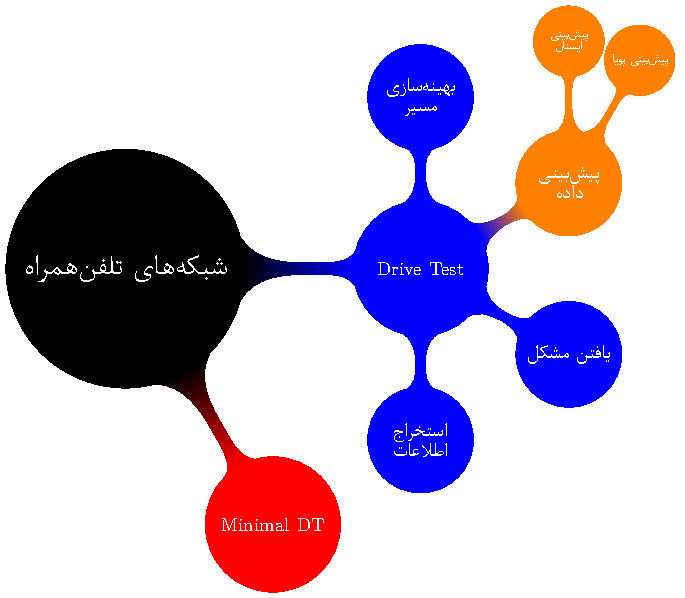
\includegraphics[width=0.65\linewidth]{Pic/plotInverseEntropy/mainFig}
\caption{\lofimage{Pic/plotInverseEntropy/mainFig}
معکوس \gls*{Entropy}
\gls*{AdversarysErrorProbability}،
تابعی است اکید صعودی.
}
\label{fig:plotInverseEntropy}
\end{figure}



\section{اثبات \autoref{lemma:calculateEntorp}}
\label{subsec:appcalculateEntorp}
$\mathrm{H}(k|Y)$
را می‌توان به صورت زیر بازنویسی نمود
\cite[بخش $2.2$]{cover2006elements}:
\begin{equation}
\mathrm{H}(k|Y) = \mathrm{H}(k,Y)-\mathrm{H}(Y).
\label{eq:conditionalEntopry}
\end{equation}
باتوجه به رابطه فوق، برای محاسبه 
$\mathrm{H}(k|Y)$
کافی است که 
$\mathrm{H}(k,Y)$ و $\mathrm{H}(Y)$
را به صورت جداگانه محاسبه کنیم. در مرحله 
\gls{Delivery}، \gls{Server}
مقدار باقیمانده فایل $A$ و $B$ را با احتمال‌های 
$P_A$ و $P_B$ برای \gls{User}
ارسال می‌کند. اگر به عنوان مثال از فایل $A$ مقدار
$N-j$
بیت در 
\gls{Cache}
ذخیره شده باشد، آنگاه در مرحله
\gls{Delivery}
می‌بایست تعداد $j$ بیت ارسال شود. به صورت مشابه چنین داستانی در مورد فایل $B$ نیز رخ می‌دهد. برای  محاسبه
$\mathrm{H}(k,Y)$، \gls{JointDistribution} $\mathrm{Pr}[k=i,Y=j]$
را برای 
$i\in \{0,1\}$, $j\in \{0,1,2,\ldots, N\}$
می‌بایست به صورت زیر محاسبه نمود. 
\begin{equation}
\mathrm{Pr}[k=i,Y=j] =\mathrm{Pr}[Y=j|k=i] \times \mathrm{Pr}[k=i],
\label{eq:urjdmk}
\end{equation}
که در آن
\begin{equation*}
\mathrm{Pr}[Y=j|k=0] = \mathrm{Pr}[Z=N-j],\quad \quad 
\mathrm{Pr}[Y=j|k=1] = \mathrm{Pr}[Z=j].
\end{equation*}
بنابراین $\mathrm{H}(k,Y)$  به صورت زیر محاسبه خواهد شد. 
\begin{align} 
\mathrm{H}(k,Y) =& -\sum_{j=0}^{N}\sum_{i=0,1}\mathrm{Pr}[k=i,Y=j] \log_2 \mathrm{Pr}[k=i,Y=j] \\
=& -\sum_{j=0}^{N} P_A\mathrm{Pr}[Z=N-j]\log_2 (P_A\mathrm{Pr}[Z=N-j]) -\sum_{j=0}^{N} P_B\mathrm{Pr}[Z=j]\log_2 (P_B\mathrm{Pr}[Z=j]). \nonumber
\end{align}
بعد از مقداری محاسبه خواهیم داشت:
\begin{align}
\mathrm{H}(k,Y)  =& -P_A\log_2 P_A - P_B\log_2 P_B 
- P_A\sum_{j=0}^{N}\mathrm{Pr}[Z=N-j]\log_2 \mathrm{Pr}[Z=N-j] \nonumber\\
& - P_B\sum_{j=0}^{N}\mathrm{Pr}[Z=j]\log_2 \mathrm{Pr}[Z=j]\nonumber\\
& = \mathrm{H}(k)+ (P_A+P_B)\mathrm{H}(Z) = \mathrm{H}(k)+\mathrm{H}(Z).
\label{eq:HXYJointgfhh}
\end{align}
در نهایت با استفاده از
 \eqref{eq:conditionalEntopry} و \eqref{eq:HXYJointgfhh}, 
 می‌توان به
  \eqref{eq:dkoclslcs}
  دست یافت. 


\section{اثبات \autoref{lemma:withoutrate}}
\label{sec:withoutrate}
برای
\gls{RandomVariable} $Y$
داریم:
\begin{equation}
\mathrm{Pr}[Y=j] = P_A \mathrm{Pr}[Z=N-j]+P_B\mathrm{Pr}[Z=j].
\label{eqPYPR}
\end{equation}
برای حل
\gls{OptimizationProblem} \eqref{eq:optmizationProblem} 
ما فرض می‌کنیم که پاسخ مساله 
\gls{UniformDistribution}
است و در ادامه اثبات خواهیم نمود که بیشینه مقدار
\gls{ObjectiveFunction}
مساله مذکور، با همین پاسخ بدست خواهد آمد. نخست این که می‌دانیم که شرط همواره 
\gls{Ambiguity}
را کم می کند
\cite[صفحه 248]{marinescu2011classical}:
\begin{equation}
\mathrm{H}(k|Y) \leq \mathrm{H}(k).
\label{eq:soskcsdcd}
\end{equation}
با استفاده از 
 \autoref{lemma:calculateEntorp} و \eqref{eq:soskcsdcd}, 
 می‌توان به نامساوی زیر دست یافت:
\begin{equation}
\mathrm{H}(Z) - \mathrm{H}(Y) \leq 0.
\label{eq:maxvalreach}
\end{equation}
برای
\gls{UniformDistribution}، $Z$
به بیشینه
\gls{Entropy}
خود یعنی
$H(Z) = \log_2 (N+1)$
خواهد رسید
\cite[قضیه $1.4.2$]{ash2012information}.
با استفاده از تعریف
\gls{Entropy} و 
\eqref{eqPYPR}  برای  $Y$ 
به 
 \eqref{eq:mathtmHY}
خواهیم رسید. 
\begin{align}
\mathrm{H}(Y)  &= -\sum_{j=0}^{N}\mathrm{Pr}[Y=j] \log_2 \mathrm{Pr}[Y=j]= -\sum_{j=0}^{N} \left(P_A \frac{1}{N+1}+P_B\frac{1}{N+1}\right)\log_2 \left(P_A \frac{1}{N+1}+P_B\frac{1}{N+1}\right)\nonumber\\
&=-\frac{1}{N+1}\sum_{j=0}^{N}\log_2 \left(\frac{1}{N+1}\right)=\log_2 (N+1).
\label{eq:mathtmHY}
\end{align}
بدین‌سان خواهیم داشت:
\begin{equation*}
\mathrm{H}(Z) - \mathrm{H}(Y) = \log_2 (N+1) - \log_2 (N+1) =0.
\end{equation*}
باتوجه به این‌که 
$\mathrm{H}(Z) - \mathrm{H}(Y)$
حداکثر مقدارش صفر است، پس می‌توان نتیجه گرفت که ما به حداکثر مقدار دست یافتیم. پس 
\gls{UniformDistribution}
پاسخ مساله ما خواهد بود. 


\section{اثبات \autoref{lemma:withrate}}
\label{sec:withrate}
فرض کنید که $Z$ از 
\gls{UniformDistribution}
پیروی کند. آن‌گاه خواهیم داشت:
\begin{equation}
\mathbb{E}[Z] = \sum_{k=0}^{N}kp_k = \sum_{k=0}^{N}\frac{k}{N+1} = \frac{N}{2}.
\label{eq:poddlicv}
\end{equation}
برمبنای 
\eqref{eq:asoksdkdcd} و \eqref{eq:poddlicv}, 
خواهیم داشت:
\begin{equation}
 \mathbb{E}[Z]=\frac{N}{2}\geq \frac{P_AN-C}{P_A-P_B} \quad \Longrightarrow \quad 
C\geq \frac{N}{2}.
\end{equation}
یعنی  در صورتی‌که
$C\geq \frac{N}{2}$
باشد،
\gls{UniformDistribution} \gls{Constraint} \gls{CommunicationCost}
را ارضا می‌کند. از سوی دیگر می‌دانیم که 
\gls{UniformDistribution} پاسخ \gls{Optimal}
مساله بدون در نظر گرفتن
\gls{Constraint} \gls{CommunicationCost}
نیز هست (مراجعه شود به
\autoref{lemma:withoutrate}).



\section{نقاط تقاطع دو منحنی}
\label{spapdpsadf}

\begin{lemma}
\label{lem:t1t2increase}
دو تابع  زیر را در نظر بگیرید.
\begin{eqnarray}
q_{1,\tau}(t) &=& \alpha_{1}h(t-\tau) \nonumber\\
q_{2,\tau'}(t) &=& \alpha_{2}h(t-\tau')
\end{eqnarray}
که در آن  $h(.)$ یک تابع 
\gls{Continuous} و \gls{StrictlyIncreasing}
است. در مورد نقاط تقاطع دو تابع 
$q_{1,\tau}(t)$ و $q_{2,\tau'}(t)$ 
می‌توان موارد زیر را برشمرد. 
\begin{itemize}
\hand
اگر 
$\tau_{1} < \tau_{2}$ و $\alpha_{1}> \alpha_{2}$
آن‌گاه این دو تابع  هیچ نقطه تقاطعی در $t>0$ نخواهند داشت. به بیان ریاضی  داریم:
\begin{equation}
\forall \tau_{1}, \tau_{2}, \alpha_{1}, \alpha_{2} \in \mathbb{R}\quad  \tau < \tau',\;  \; \alpha_{1}> \alpha_{2} \quad \quad \#\left\{ t|t = \arg \left(q_{1,\tau}(t) \cap q_{2,\tau'}(t)\right) , t \geq 0\right\} = 0
\end{equation}
\hand
اگر 
$\tau_{1} < \tau_{2}$ و $\alpha_{1}< \alpha_{2}$
آن‌گاه این دو تابع  حتما در یک نقطه در $t>0$ همدیگر را قطع خواهند کرد. به بیان ریاضی داریم.
\begin{equation}
\forall \tau_{1}, \tau_{2}, \alpha_{1}, \alpha_{2} \in \mathbb{R}\quad  \tau < \tau',\;  \; \alpha_{1}< \alpha_{2} \quad \quad \#\left\{ t|t = \arg \left(q_{1,\tau}(t) \cap q_{2,\tau'}(t)\right) , t \geq 0\right\} = 1
\end{equation}
\end{itemize}

\end{lemma}
\begin{lemmaproof}
برای اثبات مورد اول، کافی است که اثبات کنیم که در صورت وجود نقطه برخورد، این نقطه در $t>0$ قرار ندارد. بر اساس فرض ‎\gls{StrictlyIncreasing}‎ بودن تابع $h(.)$، می‌دانیم که
\begin{equation}
\forall t_{1}, t_{2}\in\mathbb{R}\quad \text{\lr{If}}\;  t_{1}<t_{2}\Longrightarrow h(t_{1})<h(t_{2})
\end{equation}
لذا با توجه به این رابطه داریم:
\begin{eqnarray}
\forall t>0,\;\tau < \tau' &\Longrightarrow& t-\tau' < t-\tau\nonumber\\
&\Longrightarrow& h(t-\tau') < h(t-\tau)\nonumber\\
\alpha_{1}> \alpha_{2} &\Longrightarrow& \alpha_{2}h(t-\tau') < \alpha_{1}h(t-\tau) \nonumber\\
&\Longrightarrow& q_{2,\tau'}(t) < q_{1,\tau}(t) 
\end{eqnarray}
از رابطه فوق بر می‌‌آید که در تمامی $t>0$ نمی‌تواند دو تابع باهم برابر شوند و لذا نقطه برخوردی بوجود نخواهد آمد.

مورد دوم لم، از دو نکته را در بردارد. اولا می گوید دو تابع حتما یک نقطه تقاطع دارند و دوما می گوید که ما تنها با یک نقطه تقاطع مواجه هستیم. برای اثبات وجود نقطه تقاطع، از برهان خلف استفاده می‌کنیم، یعنی فرض می‌کنیم که نقطه تقاطعی وجود نداشته باشد. با توجه به صعودی بودن تابع و عدم وجود نقطه تقاطع، می‌توان نتیجه گرفت که 
\begin{eqnarray}
\forall t>0,\;\tau < \tau'   &\Longrightarrow& q_{1,\tau}(t) >  q_{2,\tau'}(t)  \nonumber \\
&\Longrightarrow&  \alpha_{2}h(t-\tau') < \alpha_{1}h(t-\tau) \nonumber\\
\forall t>0,\;\tau < \tau' &\Longrightarrow& t-\tau' < t-\tau\nonumber\\
&\Longrightarrow& h(t-\tau') < h(t-\tau)\nonumber\\
\end{eqnarray}
به دلیل این‌که پارامترهای $‎\tau$ و $‎\tau'$ جزو درجات آزادی توابع محسوب می‌شوند، لذا می‌توان آن‌ها را به دلخواه انتخاب نمود و در ضمن به ازای تمامی این مقادیر باید روابط (مقداری از اثبات مانده است)

\end{lemmaproof}



\section{اثبات قضیه \ref{lemma:Mipismallthanp}}
\label{sec:Mipismallthanp}


‎\autoref{subfig:NIPismalthn}‎ 
نمایی از سناریوی مورد بحث را نشان می‌دهد. بر طبق لم بیان شده در پیوست ‎\ref{lem:t1t2increase}‎ می‌توان دریافت که دو تابع ‎‎اولویت
 $q_{p,0}(t)$ و $q_{i,-\tau}(t)$ 
 همدیگر را حتما در یک نقطه در $t>0$ قطع می‌کنند. این نقطه را با $t_{o}$ نامگذاری می‌کنیم. همان‌طور که مشاهده می‌کنید از زمان صفر تا $t_{o}$ مشتری موجود در صف با اولویت $i$ اولویتش بیشتر از $‎\xi$ است، اما بعد از زمان $t_{o}$ این رویداد تغییر می‌کند. نکته مهم در این است که اگر کل زمان انتظار مشتری در صف و یا به عبارت دیگر مدت ‎\gls{WaitingTime}‎ حداقل $‎\tau$ و حداکثر 
$t_{o} + \tau$
باشد، این مشتری زودتر از $‎\xi$ خدمات دریافت می‌کند.



بدین‌منظور ابتدا باید نقاط برخورد دو تابع اولویت را محاسبه کنیم. نقطه برخورد دو تابع را به صورت زیر محاسبه می‌کنیم.
\begin{equation}
\alpha_{p}h(\mu_i) = \alpha_{i}h(\tau+\mu_{i}),\quad\quad \alpha_i<\alpha_p.
\label{eq:kadkoddd}
\end{equation}
جواب معادله فوق را برابر با  $t_{o}$ در نظر می‌گیریم. پارامتر 
$\omega_{i}(\tau)$
را زمان انتظار مشتری در نظر می‌گیریم که  در زمان $‎‎\tau$ وارد شده است و دارای اولویت $i$ است. با توجه به ‎
‎\autoref{subfig:NIPismalthn}‎ 
 اگر مقدار مدت زمان انتظار مشتری با اولویت $i$ ام در بازه
$\tau \leq \omega_{i}(\tau)\leq \tau+ t_{o}$، 
این مشتری جزو مشتریانی محسوب می‌شود که قبل از $‎\xi$ وارد شده است، و بعد از زمان ورود او و قبل از او وارد ‎\gls{Server}‎ می‌شود. انتگرال زیر را در نظر بگیرید.
\begin{equation}
\mathbb{E}[N_{ip}] = \int_{0}^{+\infty} \lambda_{i}\mathrm{Pr}[\tau<\omega_{i}\leq \tau+\mu_i]\mathrm{d}\tau \quad i< p,
\label{dsfdsfsdfgrgr}
\end{equation}
پارامترها:
\begin{itemize}
\tree $\omega_{i}(\tau)$ :
مدت زمانی که مشتری وارد شده در زمان  $‎\tau$ در صف با اولویت ‎$i$ انتظار می‌کشد. 
\tree $\lambda_{i}$ :
نرخ ورود مشتریان به صف با اولویت $i$.
\tree $\mathbb{E}[N_{ip}]$ :
میانگین تعداد افرادی که در اولویت $i$ قرار دارند و از دیدگاه یک مشتری معین در اولویت $p$ 
($\xi$)
زودتر ‎\gls{Service}‎ دریافت می‌کنند.
\tree $t_{o}$ :
نطقه برخورد دو تابع ‎\gls{Priority}‎
$q_{p,0}(t)$ و $q_{i,-\tau}(t)$
و یا به عبارت دیگر مشتری با اولویت $i$ حداکثر تا لحظه $t_{o}$ از $‎\xi$ اولویتش بیشتر است.
\end{itemize}
در انتگرال  ‎‎\ref{dsfdsfsdfgrgr}‎ مقدار 
$\lambda_{i}\mathrm{d}\tau$
برابر با ‎\gls{Expectation}‎ تعداد مشتریانی است که در بازه 
$[-\tau-\mathrm{d}\tau , -\tau]$
وارد صف با اولویت $i$ می‌شوند. از سوی دیگر 
$\mathbb{P}[\tau<\omega_{i}(\tau)\leq g(\tau)]$
احتمال این را نشان می‌دهد که مشتری رسیده در بازه یاد شده، به مدت زمان حداقل $‎\tau$ و حداکثر $g(‎\tau)$ در صف به انتظار بنشیند. وظیفه 
$\int_{0}^{+\infty}$
نیز در نظر گرفتن تمامی مشتریانی است که در تمامی لحظات قبل از $‎\xi$ وارد صف با اولویت $i$ شده‌اند. 

انتگرال ‎\ref{dsfdsfsdfgrgr}‎ را می‌توان به صورت زیر بازنویسی کرد.
\begin{align}
\mathbb{E}[N_{ip}] &= \int_{0}^{+\infty} \lambda_{i}\mathrm{Pr}[\tau<\omega_{i}\leq \tau+\mu_i]\mathrm{d}\tau \nonumber \\
&=\lambda_{i} \int_{0}^{+\infty}\mathrm{Pr}[\omega_{i} \leq \tau+\mu_i]\mathrm{d}\tau - \lambda_{i} \int_{0}^{+\infty}\mathrm{Pr}[\omega_{i} \leq \tau]\mathrm{d}\tau\nonumber\\
&= \lambda_{i}  \underbrace{\int_{0}^{+\infty}(1-\mathrm{Pr}[\omega_{i} \leq \tau])\mathrm{d}\tau}_\text{first term}  - \lambda_{i} \underbrace{\int_{0}^{+\infty}(1-\mathrm{Pr}[\omega_{i} \leq \tau+\mu_i])\mathrm{d}\tau }_\text{second term} .
\label{eq:eintinfty}
\end{align}
لازم به ذکر است که 
$\mathbb{P}[\omega_{i}(\tau)\leq \tau]$
بیانگر 
\gls{CumulativeDistributionFunction} ‎\gls{WaitingTime}‎
  برای مشتری است که در لحظه $‎\tau$ وارد صف با اولویت $i$ شده است. به دلیل این‌که مشتریان وارد شده به صف، با فرایند پواسن  وارد صف می‌شوند، لذا تابع توزیع ‎\gls{WaitingTime}‎ مستقل از زمان ورود خود مشتری خواهد شد.
به همین دلیل می‌توان به جای  $\omega_{i}(\tau)$ از $\omega_{i}$ استفاده نمود. پس رابطه ‎\ref{eq:eintinfty} به صورت زیر تبدیل خواهد شد.
\begin{equation}
\mathbb{E}[N_{ip}] = \lambda_{i} \int_{0}^{+\infty}\left(1-\mathbb{P}[\omega_{i} \leq \tau]\right)\mathrm{d}\tau-
\lambda_{i} \int_{0}^{+\infty}\left(1-\mathbb{P}[\omega_{i}\leq g(\tau)]\right)\mathrm{d}\tau \quad i< p
\label{Eq:Nipwwitho}
\end{equation}
\gls{Expectation} \gls{RandomVariable} $\omega_{i}$
به صورت زیر تعریف می‌شود
\cite{bassett2000statistics}.
\begin{eqnarray}
W_{i} = \mathbb{E}[\omega_{i}] &=& \int_{0}^{+\infty} x f_{\omega_{i}}(x)\mathrm{d}x \nonumber\\
&=&\int_{0}^{+\infty} \left(1-F_{\omega_{i}}(x)\right)\mathrm{d}x = \int_{0}^{+\infty} \left(1-\mathbb{P}[\omega_{i}\leq x]\right)\mathrm{d}x 
\label{Eq:Ewidef}
\end{eqnarray}
که در آن 
$f(.)$ و $F(.)$
به ترتیب توابع ‎\gls{PDF}‎ و ‎\gls{CDF}‎ هستند.

با توجه به رابطه ‎\ref{Eq:Ewidef}‎ رابطه ‎\ref{Eq:Nipwwitho}‎ را می‌توان به صورت زیر بازنویسی نمود.
\begin{equation}
\mathbb{E}[N_{ip}] = \lambda_{i} W_{i}- \lambda_{i} \int_{0}^{+\infty}\left(1-\mathbb{P}[\omega_{i}\leq g(\tau)]\right)\mathrm{d}\tau \quad i< p
\label{Eq:NEWlambda}
\end{equation}
برای محاسبه قسمت دوم رابطه فوق، رویه زیر را در پیش می‌گیریم.
\begin{align}
\alpha_i(\mathrm{d}\tau + \mathrm{d}\mu_i)h'(\tau+\mu_i) & =
\alpha_p  \mathrm{d}\mu_i \times h'(\mu_i).
\end{align}

\begin{align}
\mathrm{d}u&=\mathrm{d}\tau+\mathrm{d}\tau \left(\frac{\alpha_i h'(\tau+\mu_i)}{\alpha_p h'(\mu_i)-\alpha_i h'(\tau+\mu_i)}\right) \nonumber\\
&= \mathrm{d}\tau \times \left(\frac{\alpha_p h'(\mu_i)}{\alpha_p h'(\mu_i)-\alpha_i h'(\tau+\mu_i)}\right) = K' \mathrm{d}\tau,
\label{eq:jdkonggmd}
\end{align}
که در آن 
$K'$
برابر است با 
\begin{equation}
K' = \left(\frac{\alpha_p h'(\mu_i)}{\alpha_p h'(\mu_i)-\alpha_i h'(\tau+\mu_i)}\right).
\label{eq:Kconstant}
\end{equation}
و در نهایت خواهیم داشت:
\begin{equation}
\mathbb{E}[N_{ip}] = \lambda_{i} W_{i}- \lambda_{i}KW_{i} = (1-K')  \lambda_{i} W_{i} = K \lambda_{i} W_{i} \quad\quad  i< p,
\label{Eq:NEWlambda}
\end{equation}
